% Created 2020-03-30 Mon 11:43
% Intended LaTeX compiler: pdflatex
\documentclass[a4paper, 11pt]{extarticle}
             \usepackage[utf8]{inputenc}
\usepackage[left=2cm, right=2cm, bottom=2.5cm, top=2.5cm]{geometry}
% Paquetes de matemáticas
\usepackage{amsmath, amsfonts, amssymb, commath}
\usepackage{tikz}
\usepackage{tikz-cd}
\newcommand{\tikzcircle}[2][red,fill=red]{\tikz[baseline=-0.5ex]\draw[#1,radius=#2] (0,0) circle ;}%
% Ajustes de idioma, gráficos, etc
\usepackage{adjustbox}
\usepackage{float}
\usepackage{hyperref}
\usepackage{graphicx}
\usepackage{gensymb}
\usepackage[spanish, english]{babel}
\usepackage{tikz}
\usepackage{multicol}
\usepackage{listings}
\usepackage{enumitem}
\setlist{nolistsep}
\usepackage{booktabs}
\usepackage{xcolor}
\usepackage{wrapfig}
%Fuentes.
% Alegreya tiene este toque antiguo con serifa, y la tipografía de las ecuaciones es también interesante.
% Gillius no tiene serifa, y también es equilibrada.
\usepackage[T1]{fontenc}
%\usepackage[default]{gillius}
\usepackage{newpxtext, newpxmath}
% Paquete para añadir Creative Commons al final del documento
\usepackage[
type={CC},
modifier={by-nc-nd},
version={3.0},
]{doclicense}
% Propiedades de párrafo
\setlength{\parindent}{0em}
\setlength{\parskip}{1.1em}
\renewcommand{\baselinestretch}{1.05}
\setlength\itemsep{0em}
% Definición de comandos. Muchos de ellos han surgido para Geometría, aunque se
% irá actualizando la lista. POSIBLEMENTE LO INTRODUZCA COMO COMANDOS DE ORG
\newcommand{\m}{\text{medio}}
\newcommand{\iso}{\text{Isom}}
% Para incluir mathcal en las ecuaciones. El /mathcal para Alegreya es el viejo
% y floritural estilo que odio.
\usepackage{calrsfs}
\DeclareMathAlphabet{\pazocal}{OMS}{zplm}{m}{n}
% Definición de colores agradables a la vista
\definecolor{azul}{HTML}{107896}
\definecolor{naranja}{HTML}{C2571A}
\definecolor{rojo}{HTML}{9A2617}
\definecolor{amarillo}{HTML}{BCA136}
\definecolor{verde}{HTML}{829356}
\definecolor{gris}{HTML}{909090}
\definecolor{rosa}{HTML}{F9A7B0}
\definecolor{amarillochillon}{HTML}{FBB117}
% Definición de comandos para teoremas, etc. El comando también incluye
% como argumento un texto, del estilo Teorema 3.5
\newcommand{\axioma}[1]{\textcolor{naranja}{\textbf{Axioma #1}}}
\newcommand{\tma}[1]{\textcolor{rojo}{\textbf{Teorema #1}}}
\newcommand{\propo}[1]{\textcolor{rojo}{\textbf{Proposición #1}}}
\newcommand{\defi}[1]{\textcolor{azul}{\textbf{Definición #1}}}
\newcommand{\obs}[1]{\textcolor{verde}{\textbf{Observación #1}}}
\newcommand{\ejem}[1]{\textcolor{verde}{\textbf{Ejemplo #1}}}
\newcommand{\ej}[1]{\textcolor{amarillo}{\textbf{Ejercicio #1}}}
\newcommand{\lema}[1]{\textcolor{rosa}{\textbf{Lema #1}}}
\newcommand{\cor}[1]{\textcolor{rosa}{\textbf{Corolario #1}}}
% La demostración es igual pero va con una letra más pequeña y en gris.
\newcommand{\dem}[1]{\textcolor{gris}{\small{Demostración. #1}}}
% Esto pone un triangulito de peligro para cuando algo es importante.
\newcommand{\importante}{\tikzcircle[amarillo, fill=amarillo]{4pt}\,}
% Para usar columnas emplea este trozo de código
% \begin{multicols*}{2}
% [\section{Axiomas para la geometría euclidiana plana}]
% 	\axioma{P1} Si tenemos el conjunto $\P$, denominado \textbf{plano}, y la aplicación $d:\P \times \P \rightarrow \R$ llamada \textbf{distancia}, entonces$(\P, d)$ es un espacio métrico.

\defi{2.2} Una \textbf{recta} $r \subset \P$ satisface
\begin{itemizex}
	\item $r$ contiene al menos dos puntos.
	\item Para toda terna de puntos $A, B, C$, están alineados si están en $r$.
\end{itemizex}

\axioma{P2} $\P$ contiene al menos tres puntos no alineados; y por dos puntos distintos, $A$ y $B$ de $\P$ pasa una recta, $r_{AB}$.

\defi{2.6} / \tma{2.7} Dos rectas se cortan si sólo tienen un punto en común, y si no tienen ningún punto en común, entonces se denominan \textbf{paralelas}, y se denota por $a \parallel b$. Dos rectas, o se cortan o son paralelas.

\importante\axioma{P3} Para toda recta $r \subset \P$ existe una biyección $\gamma: r \rightarrow \R$ tal que $|\gamma(X) - \gamma(Y)| = |x - y| = d(X, Y) \;\; \forall \;\; X,Y \in r$ 

\obs{2.8} Si $A, B \in r$ son distintos, entonces existe un punto $M\in r: d(A,M) = d(M,B)$ que denotamos por $\m[A,B]$ y se llama \textbf{punto medio}. Asimismo sólo existe un punto $B \in r$ tal que $B = \m[A, M]$.

\obs{2.9} Si $r$ es una recta y $P \in r$, entonces $r$ se puede dividir en dos \textbf{semirrectas}, que son los conjuntos $\{X \in r \; | \; \gamma(X) > \gamma(P)\}$ y $\{X \in r \; | \; \gamma(X) < \gamma(P)\}$.

\axioma{P4} Para toda recta $r \subset \P$ hay dos subconjuntos $H^1$ y $H^2$, denominados \textbf{semiplanos} de $r$, que verifican:
\begin{itemizex}
	\item $H^1 \cup H^2 = \P-r$
	\item Si $X,Y \in H^i$ entonces $[X,Y] \subset H^i$
	\item Si $X \in H^1$ y $Y \in H^2$ entonces $[X,Y] \cap r \neq \emptyset$.
\end{itemizex}

\defi{2.15} Sean $P, Q, R$ no alineados, entonces el triángulo $\triangle\{P,Q,R\}$, o $\triangle PQR$ está formado por los segmentos $[P,Q]$, $[Q,R]$, $[P,R]$, llamados lados, y los vértices $P,Q, R$.

\tma{2.16 [Axioma de Pasch]a} Dado un triángulo $\triangle PQR$ y una recta $r$; si $r$ corta a $[P,Q]$, entonces o corta a $[P,R]$ o a $[Q, R]$.

\defi{2.17 = 1.5} Una \textbf{isometría} en $\P$ es una biyección $g: \P \rightarrow \P$ que cumple que $d(g(X), g(Y)) = d(X,Y) \;\;\forall\;\; X,Y \in \P$.

\tma{2.18} Si $A,B \in \P$ y $g \in \iso(\P)$ entonces $g([A,B]) = [g(A), g(B)]$ y $g(r_{AB}) = r_{g(A)g(B)}$ 

\axioma{P5} Si $A_1, A_2 \in \P$ y $B_1, B_2 \in \P$ son dos pares de puntos que cumplen $d(A_1,A_2) = d(B_1,B_2)$ entonces existe $g \in \iso(\P)$ tal que $g(A_i) = B_i$. Se dice que esos pares de puntos son \textbf{congruentes}.

\axioma{P6} Para toda recta $r$ existe una isometría $\sigma$ llamada \textbf{reflexión} tal que  
\begin{itemizex}
	\item $\sigma(X) = X\iff X \in r$
	\item $\sigma \circ \sigma = \text{Id}$
\end{itemizex}


\defi{2.23} / \tma{2.25} / \cor{2.30} Una recta $l$ es \textbf{ortogonal} a $r$ si para todo $S \in l$ y para todo par de puntos $A, B$ que cumple que $M = \m[A,B]$, de modo que $l \cap r = M$, entonces se da que $d(A,S) = d(S,B)$. Se denota $l \perp_M r$. En estas condiciones, $l = \{X \in \P \; | \; d(S,A) = d(S,B)\}$, se denomina \textbf{mediatriz} de $[A,B]$. 

\begin{figure}[H]
	\centering
	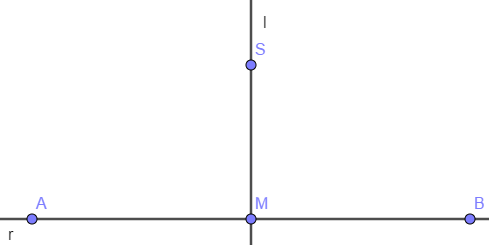
\includegraphics[width=7cm]{figuras/2-23.png}
	\vspace{-1em}
\end{figure}

\lema{2.21} Si $\sigma_r$ entonces, para todo $X$, $\m[X, \sigma_r(X)] \in r$.

\obs{2.24} Si $l \perp r$ y $g \in \iso(\P)$ entonces $g(l) \perp g(r)$.

\importante\tma{2.26} Si $l, r \subset \P$ cortan en $M$ y $\sigma_l, \sigma_r$ son dos reflexiones de $l$ y $r$, entonces se cumple que $l \perp_M r \iff r \perp_M l \iff \sigma_r(l) = l \iff \sigma_l(r) = r$.

\importante\tma{2.27 / 2.29} Para toda recta $r$ y todo punto $S \in \P - r$, existe una recta $l$ ortogonal a $r$, que pasa por $S$. Si $r$ es una recta, y $M \in r$, entonces existe $l$ tal que $l \perp_M r$.

\axioma{P7} Para toda recta $r$ y todo punto $P$ existe sólo una recta \textbf{paralela} a $r$ que pase por $P$.

\tma{2.31 / 2.33} Si $a \perp l$ y $b \perp l$ entonces $a \parallel b$. Sean $a \parallel b$. Entonces, para todo $A \in a$, la única recta $l \perp_A a$ también es ortogonal a $b$.

\tma{2.32} Las rectas parallelas forman una relación de equivalencia.
\begin{itemizex}
	\item Reflexividad: $a\parallel a$
	\item Simetría: $a \parallel b \rightarrow b \parallel a$
	\item Transitividad  $a \parallel b $ y  $b \parallel c \rightarrow a \parallel c$
\end{itemizex}

\ej{2.6} Sean $A,B \in r$, $A \neq B$. Para todo $t$, existe un único $P_t\in r$ que cumple $d(P_t,A) = \abs{t}$ y $d(P_t, B) = \abs{t-d(A,B)}$. En definitiva, la posición de $P_t$ está sólamente determinada por las distancias $d(A, P_t)$ y $d(P_t, B)$.
	 
	 
	 
	 
	 
	 
	 \end{multicols*}\pagebreak
% multicols* obliga a terminar una columna antes de empezar la siguiente.
\DeclareMathAlphabet{\pazocal}{OMS}{zplm}{m}{n}
\let\mathcal\pazocal
\usepackage{fancyhdr}
\pagestyle{fancy}
\lhead{Alex Martínez Ascensión}
\chead{}
\rhead{\today}
\date{}
\title{\Huge\vspace{-1em}Álgebra}
\hypersetup{
 pdfauthor={},
 pdftitle={\Huge\vspace{-1em}Álgebra},
 pdfkeywords={},
 pdfsubject={},
 pdfcreator={Emacs 26.2 (Org mode 9.2.5)}, 
 pdflang={English}}
\begin{document}

\maketitle
\vspace{-8em}

\section*{Anillos}
\label{sec:org4e4eff7}
\begin{multicols*}{2}

\vspace{-1.5em}
\subsection*{Generalidades}
\label{sec:org1ed9933}
\vspace{-1.5em}
\defi{1.1 (Anillo)} Un \textbf{anillo} es una estructura \((A, +, \cdot)\) con las
propiedades: \vspace{-1em}
\begin{itemize}
\item \((A, +)\) es un grupo conmutativo
\item Asociatividad: \((xy)z = x(yz)\)
\item Distributividad: \((x + y)z = xz + yz\), \(x(y+z) = xy+xz\)
\end{itemize}
Se denota al elemento unitario de \((A, +)\) por \(0_A\) y al unitario de 
\((A, +, \cdot)\), si existe, por \(1_A\). \(A^* = A/ \{ 0 \}\). \(0_A =
1_A \iff A = \{ 0 \}\).

\defi{1.6} Si \(1_A \in A\), entonces \(A\) es un \textbf{anillo unitario}. Una
\textbf{unidad} de \(A\) es un elemento \(x\) que tiene su inverso \(y\): \(xy=1\). El conjunto de unidades es \(U(A)\). El inverso, si existe, se puede denotar por \(x
^{-1}\) y \(x/y = xy ^{-1}\).

\defi{1.8} Un \textbf{cuerpo} es un anillo \(K\) tal que \(K^*\) es un grupo. O, un
anillo unitario con inverso.  

\defi{1.10} Un \textbf{divisor de cero} es un elemento \(x \in A^*\) tal que, para
algún \(y \in A^*\), \(xy = 0_A\). Un cuerpo nunca tiene divisores de cero:
\(x = x(yy ^{-1}) = (xy) y ^{-1} = 0 y ^{-1} = 0\)

\defi{1.11} Se denomina \textbf{dominio de integridad} a un anillo unitario sin divisores
de cero. El producto de dos anillos conmutativos \(C = A \times  B\) nunca es
un dominio de integridad, pues \((a, 0) \neq 1_A, (0, b) \neq 1_B\) y \((a, 0) \times (0, b) = (0, 0) = 0_C\).

A un dominio de integridad se le puede asociar un cuerpo mediante el \textbf{cuerpo de
fracciones de un dominio}. 
Dada la relación \((x,y) R (x', y') \iff xy' = x'y\), para el producto de dominios \(A \times  A^*\) 
entonces para la clase de equivalencia \([x,y]\), las operaciones \([x,y] +
[x', y'] = [xy' + y'x, yy'], [x,y]\cdot [x',y'] = [xx', yy']\) forman un
cuerpo, \(K\), con \(0_K = [0, 1]\), \(1_K = [1,1]\), y \([x,y] ^{-1} =
 [y, x]\).

\defi{1.14 (Ideal)} Un \textbf{ideal} es un subconjunto \(I \subset A\) tal que \vspace{-1em}
\begin{itemize}
\item \(I\) es subgrupo de \(A\)
\item \(\forall i \in I, a \in A, ia \in I\).
\end{itemize}
\(A, \{ 0 \}\) son los \textbf{ideales triviales}, y si \(I \neq A\), \(I\) es un  
\textbf{ideal propio}. Si \(1_A \in I\), \(I = A\): \(\forall a \in A\), \(a = a
\cdot 1\), y como \(1 \in I, a \in I\).

\defi{1.16} Dado un ideal \(I\) de \(A\), dada la relación \(xRy \iff x-y
\in I\), se forma el \textbf{anillo cociente} \(A/I\) con las clases de equivalencia
\([x] = x + I = \{ x + a \;|\; a \in I  \}\).
Las operaciones suma y producto definidas por \((x + I) + (y + I) = (x + y) +
I, \; (x + I)(y + I) = xy + I\), son inyectivas.

\defi{1.17 - 1.19} Sea \(A\) un anillo conmutativo y \(L\) un subconjunto de \(A\). El conjunto \(I\) de sumas finitas \(a_1x_1 + ... + a_lx_l,\; a_i \in A,
l_i \in L\) es un \textbf{ideal generado por \(L\)}. Además, \(I\) es el mínimo 
ideal que contiene a \(L\). Si \(L\) es finito, \(I\) es \textbf{finitamente generado}; y si \(L\) tiene
un solo elemento, es decir, \(I = Al\), el ideal es \textbf{principal}.

En los ideales se definen la (1) suma: \(I + J\) está dado por \(a_1, \cdots,
a_r, b_1, \cdots, b_s \in A, x_1, \cdots, x_r \in I, y_1, \cdots, y_s \in J,
a_1x_1 + \cdots + a_rx_r + b_1y_1 + \cdots + b_sy_s = x + y\); (2) producto: IJ
= \(x_1y_1 + \cdots + x_ry_r, x_1, \cdots, x_r \in I, y_1, \cdots, y_r \in J\), (3) intersección \(I \cap J\).

\ejem{1.20.2} En un cuerpo \(K\) sólo son ideales \(\{0\}\) y \(K\). Si \(I\) es ideal no trivial de \(K\), para \(x \in I \ \{0\}\) existe \(x^{-1} \in
K\) y \(1 = xx^{-1} \in I\), y \(I\) es ideal impropio. $\backslash$)

\defi{1.21} Un ideal es \textbf{maximal} si (1) \(A/I\) es un cuerpo y (2) \(I\) es
propio y ningún otro ideal propio lo contiene. \((1) \iff (2)\).
\textcolor{gray}{\footnotesize Si \( A/I  \) es
un cuerpo, luego contiene una unidad. Ninguna unidad \( i \) de \( A/I  \) puede estar
en \( I^* = I + i \) porque entonces \( I^* = A \)}.

\defi{1.22} Sean \(A\) unitario e \(I\) un ideal. Se dice que \(I\) es
\textbf{primo} si (1) \(A/I\) es un dominio de integridad y (2) \(I\) es propio, y
\(\forall x,y \in A\), si \(xy \in I\), \(x \in I\) o \(y \in I\). \((1) \iff (2)\).
\dem{ Si \( xy \in I  \), \( 0 + I = xy + I = (x+I)(y+I) \). Como \( A/I  \) es dominio, 
\( x+I = 0 + I \rightarrow x \in I \) o \( y+I = 0 + I \rightarrow y \in I  \).  }

\defi{1.24} Un \textbf{homomorfismo} de los anillos \(A,B\) es una aplicación \(f: A
\rightarrow B\) definida por: \vspace{-1em}
\begin{itemize}
\item \(f(x+y) = f(x) + f(y)\)
\item \(f(xy) = f(x)f(y)\)
\item \(f(1_A) = 1_B\)
\end{itemize}
\vspace{-1em}\textcolor{gray}{\footnotesize \( f(x) (f(1_A) - 1_B) = f(x)f(1_A) - f(x)1_B = f(x\cdot 1_A) - f(x) = 0 \). 
Si \( f(1_A) \neq 1_B \), f(A) son divisores de 0.}
La aplicación composición \(\phi: A \rightarrow A: g \mapsto g \circ f\) es
homeomorfismo. 

\defi{1.26 (Núcleo e imagen)} Se define el \textbf{núcleo} de \(f\) al ideal: \(\text{ker } f
= \{ x \in A \;|\; f(x) = 0 \}\), y se define la \textbf{imagen} de \(f\) al anillo \(\text{im } f = \{ y \in B \;|\; \exists x \in A, f(x) = y \}\).

\propo{1.27 / 1.30} \textbf{Teorema de isomorfía}. Dado un homomorfismo \(f\), el diagrama

\ejem{1.31} Si \(f: K \rightarrow  B\) es homomorfismo de anillos unitarios
conmutativos y \(K\) es un cuerpo, entonces \(f\) es monomorfismo, pues \(\text{ker } f = \{ 0 \}\) es ideal propio.
\vspace{-1em}
\begin{center}
\begin{tikzcd}
A \ar{r}{f} \ar{d}{p}        & B                            \\
A/\text{ker } f \ar{r}{\overline{f}} & \text{im } f \ar{u}{j}
\end{tikzcd}
\end{center}
\vspace{-1em}
Con \(p: x \mapsto x + \text{ker }f\) sobreyectiva / \textbf{epimorfismo}, \(\overhead{f}: x +
\text{ker }f \mapsto f(x)\) biyectiva / \textbf{isomorfismo}, \(j: y \mapsto y\)
inyectiva / \textbf{monomorfismo}; es
conmutativo.  
Si \(f\) es monomorfismo entonces \(\text{ker }f = \{ 0 \}\). Dos anillos
conmutativos son \textbf{isomorfos} (\(A \simeq B\)) si existe un isomorfismo entre
ellos.
\vspace{-1.5em}
\subsection*{Divisibilidad}
\label{sec:org7b5c89c}
\vspace{-1.5em}
\defi{2.1} \textbf{x es un divisor de y} o \textbf{y es un múltiplo de x}, \(x | y\) si existe
\(a \in A, y = ax\). Si \((x) = \{ kx \;|\; k \in \mathbb{Z} \}\), entonces
\(x|y \iff (y) \subset (x)\). \(x\) \textbf{está relacionado con} \(y\) si \((x) =
(y) \iff x|y, y|x\). En ese caso, existe una unidad \(a \in U(A)\) tal que \(y = ax\).
\vspace{-1em}\textcolor{gray}{\footnotesize Si \( (y) = (x), y \in(x), x \in(y); y = ax, x = by. y = aby \iff 1 = ab \).}

Denotamos \(\text{div } (y)\) al conjunto de divisores de \(y\). Si \(y\)
genera un ideal primo, entonces decimos que \(y\) \textbf{es primo}. \(y\) es
\textbf{irreducible} si sus divisores son las unidades y productos de \(y\) por
unidades. 
\textbf{Todo primo es irreducible}, pero \textbf{NO TODO irreducible es primo} (hay irreducibles
que no generan ideales primos).

\defi{2.6} Se dice que \(A\) es un \textbf{dominio euclídeo \textcolor{red}{DE}} 
si existe una aplicación \(\left\Vert \cdot \right\Vert : A \rightarrow
\mathbb{N}\) tal que \vspace{-1em}
\begin{itemize}
\item \(\left\Vert x \right\Vert = 0 \iff x = 0\)
\item \(\left\Vert xy \right\Vert  = \left\Vert x \right\Vert \cdot \left\Vert y \right\Vert\)
\item Si \(x,y \in A^*\) existe \(r \in A\) tal que \(y |(x-r)\) y \(\left\Vert r \right\Vert < \left\Vert y \right\Vert\)
\end{itemize}
\vspace{-1em}\textcolor{gray}{\footnotesize \( \mathbb{Z} \) es DE porque el valor absoluto cumple la función. 
En \( \mathbb{Z}[i] \) la función \( \left\Vert a+ bi \right\Vert = a^2 + b^2 \) cumple las propiedades y \( \mathbb{Z}[i] \) es DE.
}

\propo{2.8} Si \(A\) es DE, entonces \(U(A) = \{ x \in A \;|\; \left\Vert x
\right\Vert = 1 \}\). 
\textcolor{gray}{\footnotesize \( \rightarrow) \( \left\Vert 1_A \right\Vert  = 1 \) porque 
\( \left\Vert 1_A \right\Vert = \left\Vert 1_A\cdot 1_A \right\Vert = \left\Vert 1_A \right\Vert \left\Vert 1_A \right\Vert \), y como \( \left\Vert 1_A \right\Vert \neq 0, \left\Vert 1_A \right\Vert  = 1 \).
Si \( x \in A \), existe \( x ^{-1} \) y \( \left\Vert x \right\Vert \left\Vert x ^{-1} \right\Vert = \left\Vert xx ^{-1} \right\Vert = 1 \) 
y como \( \left\Vert x \right\Vert \in \mathbb{N} , \left\Vert x \right\Vert = \left\Vert x ^{-1} \right\Vert = 1 \)}

\propo{2.10}/\defi{2.11} En un \textbf{dominio de ideales principales \textcolor{red}{DPI}}
todos los ideales son principales. Un DE es un DIP. 
\textcolor{gray}{\footnotesize Elegimos \( x \) tal que \( \left\Vert x \right\Vert = \text{min}\{ \left\Vert y \right\Vert  \;|\; 0 \neq y \in I  \} \). 
Entonces \( x > 0 \) y \( I  \) está generado por \( x \), ya que si \( y \neq 0, y \in I  \),
existe \( r \in A \) tal que \( x|(y-r), \left\Vert r \right\Vert < \left\Vert x \right\Vert  \). Entonces \( y-r \in I  \) y como \( y \in I  \),
\( r \in I \), pero como \( \left\Vert r \right\Vert < \left\Vert x \right\Vert  \), y \( \left\Vert x \right\Vert  \) es el mínimo en \( I  \), r = 0 y \( y \in (x) \).}

\propo{2.12} Si \(A\) es un DIP, todo elemento irreducible \(a \in A^*\)
genera un ideal maximal. 
\textcolor{gray}{\footnotesize Sea \( I  \), \( (a) \subset I  \). Entonces \( I = (a) \) o 
\( I = A \). Sea \( b \in A \) tal que \( I = (b) \). Entonces \( (a) \subset I = (b), b | a \). 
Como \( a \) es irreducible, o bien \( b = ua, u \in U(A) \), y (a) = (b) = I \) o \( b \in U(A) \), y I = (b) = A.}

\defi{2.13 (Característica de un dominio de integridad)} Definimos \(\phi =
\phi_A: \mathbb{Z} \rightarrow A: k \mapsto k\cdot 1_A = 1_A + \cdots + 1_A\; (k >
0), 0\; (k = 0), -((-k) \cdot 1_A)\; (k < 0)\). \(\phi\) es un homomorfismo.
Si \(\text{ker }\phi = \{ 0 \}\), \(\mathbb{Z} \subset A\), y tiene
característica 0; y si \(\text{ker }\phi \neq \{ 0 \}\), \(A\) tiene
característica positiva. En este caso, como \(A\) es dominio de integridad y
\(Z/\text{ker }\phi \simeq \text{im } A \subset A\), \(Z/\text{ker } \phi\)
también es dominio y \(\text{ker }\phi = (p)\) es un ideal primo.

\defi{2.14} Sean \(x,y \in A^*, z \in A\). \(z\) es un \textbf{máximo común divisor}
si \(z|x, \; z|y\), y \(z\) divide cualquier otro divisor de ambos. 
\(z\) es un \textbf{mínimo común múltiplo} si \(x|z, \; y|z\) y \(z\) divide a
cualquier otro múltiplo de ambos. Estos elementos son únicos.

\propo{2.17 / 2.18 / 2.19}. Para un dominio de integridad \(A^*\): \vspace{-1em}
\begin{itemize}
\item \(\forall x,y \in A^*\) tiene mcd: \((x) + (y) \subset (mcd)\).
\item \(\forall x,y \in A^*\) tiene mcm: \((x) \cap (y) = (mcm)\).
\item xy = mcm\(\cdot\) mcd.
\end{itemize}
\textbf{Si se cumple cualquiera de los dos primeros puntos} \textbf{\textcolor{red}{MC}} , 
\textbf{todo elemento irreducible es primo \textcolor{red}{P}} . 

\propo{2.20} (\textbf{Identidad de Bezout \textcolor{red}{B}}). Si \(x,y \in A^*\) 
generan un ideal principal, existe \(z = mcd(x,y)\) y existen \(a,b \in A\) 
tales que \(z = ax + by\).

\defi{2.21} Dos elementos \(x,y \in A^*\) son primos entre sí si no comparten
más divisores que las unidades, es decir, \(mcd(x,y) = 1_A\).

\defi{2.23} Un dominio de factorización única, \textbf{\textcolor{red}{DFU}}, es un
dominio de integridad donde todo elemento irreducible es primo
(\textbf{\textcolor{red}{P}}) y todo elemento no unitario es producto de elementos
irreducibles (\textbf{\textcolor{red}{F}}).

\vspace{-1em}
\begin{center}
\begin{tikzcd}
DE \ar{r} & DIP \ar{r}\ar{d} & DFU \ar{r}\ar{d} & F \\
 & B \ar{r} & MC \ar{r} & P \\
\end{tikzcd}
\end{center}
\vspace{-1em}
\vspace{-2em}
\propo{2.26 Ecuaciones diofánticas lineales con dos incógnitas.} Las ecuaciones 
son de la forma \(\textcolor{blue}{c = aX + bY}\), de un dominio. Si se cumple la identidad de 
Bezout, y \(d = \text{mcd}(a, b)\), entonces se cumple que \(\textcolor{orange}{ d = \alpha a +
\beta b }\). Por tanto, existen \(a_0, b_0, c_0 \in A\) tales que \(\textcolor{brown}{c = c_0d},
\textcolor{brown}{a = a_0d},\textcolor{brown}{ b = b_0d}\), y \(\textcolor{orange}{ 1 = \alpha a_0 + \beta b_0 }\),
de modo que la nueva ecuación a resolver es \(\textcolor{blue}{c_0 = a_0X +
b_0Y)\).

Multiplicando por \(\alpha\) y sustituyendo \(\alpha a_0 = 1 - \beta b_0\)
tenemos \(X = \alpha c_0 + b_0 (\beta X - \alpha Y)\). Igualmente,
multiplicando por  \(\beta\) y sustituyendo \(\alpha a_0 = 1 - \beta b_0\)
tenemos \(Y = \beta c_0 - a_0 (\beta X - \alpha Y)\). Así, si \(t = \beta x -
\alpha y\), para algunos \(x,y\), 
tenemos las ecuaciones \(\textcolor{rojo}{ x = \alpha c_0 + b_0 t};  \textcolor{rojo}{ y = \beta c_0 - a_0 t}\).

Así, primero hallamos \(\textcolor{orange}{ d = \alpha a +
\beta b }\), con lo cual obtenemos \(\alpha, \beta, a, b\), y de ahí sacamos
\(\textcolor{brown}{a_0 = a / \text{mcd}}\), \(\textcolor{brown}{b_0 = b /
\text{mcd}}\), \(\textcolor{brown}{c_0 = c/\text{mcd}}\). Para obtener  \(\textcolor{orange}{ d = \alpha a +
\beta b }\) empleamos el algoritmo de Euclides.

\propo{2.27 Algoritmo de Euclides.} Este algoritmo sólo es válido en DIPs, ya
que en ellos se da B y MC. Ponemos un ejemplo práctico con \(4329 / 132\):

\(\textcolor{red}{4329} = \textcolor{orange}{132} \cdot 32 +
\textcolor{amarillo}{105}, \qquad
\textcolor{orange}{132} = \textcolor{amarillo}{105} \cdot 1 + \textcolor{green}{27}, \qquad
\textcolor{amarillo}{105} = \textcolor{green}{27} \cdot 3 + \textcolor{blue}{24}, \qquad
\textcolor{green}{27} = \textcolor{blue}{24} \cdot 1 + \textcolor{violet}{8}, \qquad
 \textcolor{blue}{24} = \textcolor{violet}{8} \cdot \textcolor{gray}{3}\)

Si tenemos la ecuación diofántica \(4329X + 132Y = 33\), vemos que tiene
solución pues \(\text{mcd}(4329, 132) = 3\) y \(3 | 33\). Para encontrar las
soluciones primero necesitamos reconstruir la ecuación  \(\textcolor{orange}{ d = \alpha a +
\beta b }\), con \(a = 4329, b = 132\). Para ello vamos sustituyendo el cociente de cada una de las
ecuaciones por la siguiente. 

\(\textcolor{red}{a} = 32\textcolor{orange}{b} +
\textcolor{amarillo}{x_2} \iff \textcolor{amarillo}{x_2} = \textcolor{red}{a} -
32\textcolor{orange}{b} \;\;||\;\;\)
\(\textcolor{orange}{b} = \textcolor{amarillo}{x_2} +
\textcolor{green}{x_3} \iff \textcolor{green}{x_3} = \textcolor{orange}{b} -
\textcolor{amarillo}{x_2} \;\; || \;\;\)
\(\textcolor{amarillo}{x_2} = 3 \textcolor{green}{x_3}+
\textcolor{blue}{x_4} \iff  \textcolor{blue}{x_4} = \textcolor{amarillo}{x_2} -
3\textcolor{green}{x_3}\) 

Finalmente, \(\textcolor{gray}{3} = \textcolor{green}{x_3} -
\textcolor{blue}{x_4}\). De aquí empezamos a sustituir todas las secuencias, al
reves, hasta llegar con \(a, b\). \(\textcolor{gray}{3} = \textcolor{green}{x_3} -
\textcolor{blue}{x_4} = 4 \textcolor{green}{x_3} - \textcolor{amarillo}{x_2} =
4\textcolor{orange}{b}  - 5\textcolor{amarillo}{x_2} = 164
\textcolor{orange}{b} - 5\textcolor{red}{a}\). Luego \(\textcolor{gray}{3} = 164
\textcolor{orange}{b} - 5\textcolor{red}{a} = \beta b + \alpha a\). Así, \(\beta = 164, \alpha = -5\). Si, además, \(a_0 = a/\text{mcd} = 4329 / 3 = 1443\),  \(b_0 = b/\text{mcd} = 132 / 3 = 44\),  \(c_0 = c/\text{mcd} = 33 / 3 = 11\), tenemos las ecuaciones  \(\textcolor{rojo}{ x = -5 \cdot 11 + 44 t};  
\textcolor{rojo}{ y = 164 \cdot 11 - 1443 t}\).

\propo{3.7 (Teoreama chino del resto)} Si \((a,b)\) son enteros primos entre
sí, \(\mathbb{Z} / ab \mathbb{Z} = \mathbb{Z} / (ab) \simeq \mathbb{Z}/(a)
\times \mathbb{Z}/(b)\). Así, el sistema de congruencias \(X \equiv m \text{ 
mod } a \;;\; X \equiv n \text{ mod } b\).

\propo{3.8} Sean \(n > 1\) y \(k \in \mathbb{Z}\). Son equivalentes:
\begin{itemize}
\item \([k] \in U(\mathbb{Z} / (n))\)
\item \(\text{mcd}(k,n) = 1\)
\item \([k] \neq 0\) y \(k\) no es divisor de cero en \(\mathbb{Z}/(n)\).
\end{itemize}

\defi{3.9 (Identidad de Euler)} Sea \(m\) positivo. Definimos \(\phi (m)\)
como el número de enteros coprimos con \(m\).
\begin{itemize}
\item \(\phi(ab) = \phi(a)\phi(b) \iff \text{mcd}(a,b) = 1\)
\item \(\phi(p^a) = p^a - p^{a-1} = p^a(1- 1/p)\) si \(p\) primo
\item \(\phi(m) =  m \prod_{i=1}^{s}(1-1/p_i)\)
\end{itemize}

\(\propo{3.12}\) Para cada entero \(n\), \(n= \sum _{d|n, d \ge 1}^{}
\phi(d)\).
\textcolor{gray}{\footnotesize Consideramos el grupo aditivo \( H = \mathbb{Z}/(n) \), 
que es cíclico de orden \( n \). Para \( 1 \le d \le n \), \( H_d \) es el cjto de elementos 
de \( H \) con orden \( d  \). Por el Tma de Lagrange, para ser \( H_d  \) subgrupo, \( d | n \).
Además, para cada \( d \) \( H_d  \) es disjunto (dos elementos diferentes no pueden tener el mismo orden),
luego \( H = \cup_{d|n} H_d \). Finalmente, se puede demostrar que \( o(H_d) = \phi(d) \).}

\propo{3.13, 3.14 (Euler, p. t. de Fermat)} Si \(\text{mcd}(k,n) = 1\), \(k^{\phi(n)} \equiv 1 \text{ mod } n\). Si \(p\) es primo, \(k^{p-1} \equiv 1
\text{ mod } p\).
\textcolor{gray}{\footnotesize Basta ver que \mathbb{Z}^*_n tiene \( \phi(n) \) 
elementos, luego si \( \text{mcd}(k,n) = 1 \), o(k) = o(\mathbb{Z}^*_n) = \phi(n) y \( k^{\phi(n)} = 1 \).}

\propo{3.15 (Teorema de Wilson)} Sea \(p\) primo. Entonces \((p-1)! \equiv -1
\text{ mod } p\). 
\textcolor{gray}{\footnotesize Demo basada en el libro de EA, que me gusta más.
(\mathbb{Z}/p \mathbb{Z}, \cdot)\) es grupo. Quitando \( [1], [-1] \), \( o([a]) \) > 2,
ya que [a][b] \equiv - 1 \text{ o } 1 \iff a = (p+1), b = (p-1) o (p+1) \). Como \( o(x) = o(-x) \),
para cada \( [a] \) existe un \( [b] \) tal que \( [a][b] = [1] \), y denotamos a ese cjto \( M \).
Entonces, \( M = \{ [2], [p-2], [3], [p-3], \cdots, [(p-1)/2], [(p+1)/2] \} \) y
\( [p-1]! = [p-1]([p-2]!) = [p-1][1] = [-1][1] = [-1] \) y \( (p-1)! \equiv -1 \text{ mod } p \).  }

\cor{3.16} Sea \(p \neq 2\) primo. Entonces si \(q = (p-1)/2\), \((q!)^2
\equiv (-1)^{q+1} \text{ mod } p\).

\end{multicols*}
\pagebreak

\section*{Polinomios}
\label{sec:orga1c709d}
\begin{multicols*}{2}
\vspace{-1.5em}
\subsection*{Generalidades}
\label{sec:org388ff8c}
\vspace{-1.5em}
\defi{1.1} Un polinomio es una construcción que necesita un anillo conmutativo
unitario \(B\) y un subanillo \(A\). Cada elemento \(f\) de \(B\) se
escribe como la suma \(f = \sum _{v = (v_1, \cdots, v_n)}^{}a_vX_1^{v_1}\cdots 
X_n^{v_n}\) donde cada \(X_i \in B\) y \(a \in A\). \(v = (v_1, \cdots,
v_n)\) son las posibles combinaciones distintas de cero de los exponentes para
las variables \(X_i\). Este anillo se denomina \textbf{anillo de polinomios en \(n\) 
indeterminadas con coeficientes en \(A\)} y se representa por \(A[X_1, \cdots,
X_n]\).

Los polinomios cumplen la unicidad, y pueden sumarse y multiplicarse de la
siguiente manera:
\[ f + g = \sum _{v}^{}(a_v + b_v) X_1^{v_1}\cdots X_n^{v_n} \]
\[ fg = \sum _{v}^{}\left( \sum _{v = \lambda + \mu}^{}a _\lambda b_\mu \right) 
X_1^{v_1}\cdots X_n^{v_n} \]
\defi{1.4} Si \(\phi: A \rightarrow A'\) es un homomorfismo entre anillos,
entonces \(\phi\) induce un anillo entre polinomios: \(\Phi: A[X_1, \cdots,
X_n] \rightarrow  A'[X_1, \cdots, X_n]\) tal que \(\sum _{v}^{}a_v
X_1^{v_1}\cdots X_n^{v_n} \rightarrow  \sum _{v}^{}\phi(a_v) X_1^{v_1}\cdots
X_n^{v_n}\). Además, \(\Phi\) es epi/monomorfismo ssi lo es \(\phi\).

\defi{1.5} Evaluación de polinomios. Dado un polinomio \(f\), y dados \(x_1,
\cdots, x_n \in B\), definimos la evaluación de un polinomio como \(ev: A[X_1,
\cdots, X_n] \rightarrow B; f(x_1, \cdots, x_n) = \sum _{v}^{}a_v x_1^{v_1}
\cdots x_n ^{v_n}\).

El teorema de isomorfía garantiza que \(A[X_1, \cdots, X_n]/ \text{ker }(ev)
\simeq A[x_1, \cdots, x_n]\). Los \textbf{ceros} de \(f\) son los elementos del núcleo
(\(f(x_1, \cdots, x_n) = 1_B\)), y en polinomios de una variable (\(A[T]\))
se llaman \textbf{raíces}.

\defi{1.5.3} Sustitución. Los polinomio permiten el cambio de unas variables \(x_1, \cdots, x_n\) a unas nuevas \(h_1, \cdots, h_n\). Por ejemplo, si
denotamos \(t = a + T\) en \(A[T]\), entonces podemos definir la sustitución
\(\phi_a: \; A[T] \longrightarrow A[T] \;;\; f \mapsto f(a+T)\). 

\defi{1.5.4} Los ideales de un polinomio son de la forma \((X_i): A[X_1,
\cdots, X_n]; x_j = {X_j \text{ si } j \neq i, 0 \text{ si } j = i\), es
decir, cuando eliminamos una de las variables. Así, \(A[X_1, \cdots, X_n]/(X_i)
\simeq A[X_1, \cdots, X_{i-1}, X_{i+1}, \cdots, X_n]\).

\defi{1.6} Funciones polinomiales. Sea \(f =  A[X_1,
\cdots, X_n]\). Se define una \textbf{función polinomial}, \(F: \; B \times \cdots
\times B \longrightarrow B ;\; (x_1, \cdots, x_n) \mapsto f(x_1, ..., x_n)\).  

\defi{1.7} Dado un polinomio no nulo \(f = \sum _{v = (v_1, \cdots, v_n)}^{}a_vX_1^{v_1}\cdots 
X_n^{v_n}\) se define el \textbf{grado} del polinomio, \(\partial f\), a la máxima
suma de exponentes de variables, es decir, \(\text{máx}(d) | v_1 + \cdots + v_n = d, a_v
\neq 0\). El \textbf{grado parcial} es \(\partial_i f: \text{máx}(d) | v_i = d\), es
decir, el exponente más alto de la variable \(X_i\). Por convenio, \(\partial
0 = \partial_i 0 = - \infty\). Se verifica que \(\partial(f+g) \le
\text{máx}(\partial f, \partial g)\) y \(\partial (fg) \le \partial f + \partial
g\). Ídem para grados parciales. 

En polinomios de una variable \(f = a_0 + a_1T + \cdots + a_nT^n\), el
\textbf{coeficiente director} es \(a_n\). Si \(a_n = 1\), decimos que \(f\) es
\textbf{mónico}. 

\defi{1.8} Dado un polinomio \(f\) de grado \(p\), las \textbf{componentes
homogéneas}, \(f_0, f_1, \cdots, f_p\) son los sumandos de igual grado total.
Los \textbf{monomios} son las componentes homogéneas de un solo sumando, \(a_vX_1^{v_1} \cdots
X_n^{v_n}\). Dadas dos formas homogéneas de grados \(p\) y \(q\), su
producto tiene grado \(p + q\).

\propo{1.9}/\cor{1.10} \(A[X_1, \cdots, X_n]\) es dominio de integridad ssi lo
es \(A\). Entonces \(\partial(fg) = \partial f + \partial g\).

\cor{1.11} Si \(A\) es dominio, \(U(A) = U( A[X_1, \cdots, X_n])\). 
\textcolor{gray}{\footnotesize Si \( a \in U(A)\), existe \( a^{-1} \) en \( U(A) \),
 y es inverso en \(  A[X_1, \cdots, X_n] \), luego \( a \in U( A[X_1, \cdots, X_n]) \). 
 Por otra parte, si \( f \in U(A[X_1, \cdots, X_n]) \), existe \( g \) tal que \( 1 = fg \), y 
\(0 = \partial1 = \partial(fg) = \partial f+ \partial g \iff \partial f = \partial g = 0\), luego \( f \in U(A)  \).}

\defi{1.12.2} El cuerpo \(K(X_1, \cdots, X_n)\) es el \textbf{cuerpo de funciones 
racionales} con coeficientes en \(K\) en \(n\) indeterminadas, y sus
elementos vienen dados como \(f / g; f,g \in K[X_1, \cdots, X_n]\), donde \(K\) es el cuerpo de fracciones de \(A\). Así, cada elemento \(f/g\) es de la
forma \(\sum _{\lambda}^{}a_\lambda X_1^{\lambda_1} \cdots X_n^{\lambda_n} /
\sum _{\mu}^{}b_\mu X_1^{\mu_1} \cdots X_n^{\mu_n}\).

\defi{1.13} \textbf{Derivación}. Dado un anillo \(A[T]\), la derivada de un polinomio
\(f = a_0 + a_1T + \cdots + a_p T^p\) es el polinomio \(\frac{\partial
f}{\partial T}= a_1 + \cdots + pa_pT^{p-1}\). Se comprueba que \(\frac{\partial
(f+g)}{\partial T} = \frac{\partial f}{\partial T} + \frac{\partial g}{\partial
T}\) y \(\frac{\partial fg}{\partial T} = f \frac{\partial g}{\partial T} + g
\frac{\partial f}{\partial T}\). 
\vspace{-1.5em}
\subsection*{División de polinomios}
\label{sec:orga4bb7e7}
\vspace{-1.5em}
\lema{2.1} Sea \(g \in A[T]\) y \(a \neq 0\) su coeficiente director.
Entonces para cualquier \(f \in A[T]\) existen \(Q, R \in A[T]\) únicos tales que
\(a^rf = Qg + R\) y \(\partial R < \partial g\); siendo \(r = \text{max}(0,
\partial f - \partial g + 1)\).

\cor{2.2 Regla de Ruffini}. Sea \(c \in A\) fijo. Para cada \(f \in A[T]\)
existe un \(Q \in A[T]\) tal que \(f = Q(T-c) + f(c)\). En particular, \((T-c)|f \iff f(c) = 0\). 
\textcolor{gray}{\footnotesize Aplicando \( g = T-c \) obtenemos \( f = Q(T-c) + 
R \), y como \( \partial R < \partial g = 1 \), \( \partial R = 0 \) y \( R \in A \). Evaluamos la expresión en 
\( c \) y tenemos \( f(c) = Q(c)(c-c) + R(c) = R \) y resulta el lema.}

\cor{2.3} Un polinomio no nulo \(f \in A[T]\) tiene a lo sumo \(\partial f\)
ceros distintos en \(A\).

\cor{2.4} Sea \(A\) un dominio infinito. Sean \(f,g \in A[X_1, \cdots, X_n]\) dos polinomio tal que existe otro \(l \in A[X_1, \cdots, X_n]\) tal que
para todo \((x_1, \cdots, x_n)\), \(f(x_1, \cdots, x_n) \neq 0\), y \(f(x_1, \cdots, x_n) = g(x_1, \cdots, x_n)\), entonces \(f=g\).

\lema{2.5} Para los polinomios \(A[T]\) la aplicación \(|| \cdot || : \; A[T]
\longrightarrow \mathbb{N} \;;\; f \mapsto || f || = 2^{\partial f}\) define a
\(A[T]\), \textbf{si \(A\) es cuerpo}, como DE.

\propo{2.6} \(A\) es cuerpo \(\iff\) \(A[T]\) es DE \(\iff\) \(A[T]\)
es DIP.

\propo{2.7} \(A\) es DFU \(\iff\) \(A[T]\) es DFU \(\iff\) \(A[X_1,
\cdots, X_n]\) es DFU.

\defi{2.10.1} Se llama \textbf{contenido} de un polinomio \(f \in A[T]\) y se denota
por  \(\textbf{c}f\), al máximo común divisor de sus coeficientes. Así, \(\textbf{c}(f)|f\) y \(f = \textbf{c}(f)f_1\).

\obs{2.11} Un polinomio \(f \in A[T]\) con contenido 1 es irreducible en \(A[T]\) ssi lo es en \(K[T]\).

\propo{2.13} (simplificada). Sea \(A\) dominio y \(f \in A[T]\), con grado
\(n\). Entonces existe un cuerpo \(L \supset A\) y elementos \(a_0, x_1,
\cdots, x_n \in L\) tales que \(f = a_0(T - x_1)\cdots(T-x_n)\). 
\vspace{-1.5em}
\subsection*{Factorización}
\label{sec:orgf6701cf}
\vspace{-1.5em}
   \propo{3.2 (Factorización de Kronecker)} Sea \(f \in A[T]\), \(A\) de 
característica 0 y \(U(A)\) es finito, \(\textbf{c}(f) = 1\), \(\partial f
> 0\) y sea \(s\) el mayor entero \(\le \partial f / 2\). Entonces la
factorización, si existe, se da en los siguientes pasos:
\begin{itemize}
\item Elegir \(s+1\) elementos distintos \(n_0, ..., n_s\) tales que \(f(n_0),
  f(n_1), \cdots, f(n_s) \neq 0\).
\item Creamos, para cada \(n_i\), el conjunto de divisores \(D_i\) en \(A\) de
\(f_(n_i)\), y establecemos \(D = D_0 \times \cdots \times D_s\).
\item Para cada \(M = (m_0, \cdots, m_s) \in D\) creamos el polinomio
\end{itemize}
\[ f_M = \sum _{k}^{s}m_k \prod_{l \neq k}^{s}\frac{T - n_l_}{n_k - n_l} \in K[T]c
\]
\begin{itemize}
\item Si \(f_M | f\), hemos encontrado un polinomio divisor. Si ningún \(f_M\)
es divisor de \(f\), \(f\) es irreducible.
\end{itemize}

\propo{3.4} Sea \(f \in K[T]\), \(2 \le \partial f \le 3\). Entonces \(f\)
es reducible ssi \(f\) tiene alguna raíz de en \(K\).

\propo{3.5} Sea \(f = a_0 + a_1T + \cdots + a_pT^p \in A[T], a_p \in U(A)\).
Entonces toda raíz en \(K\) está en \(A\) y es divisor de \(a_0 = f(0)\)
en \(A\).

\propo{3.7 (Eisenstein)} Sea \(f = a_0 + a_1T + \cdots + a_pT^p \in A[T]\) con
contenido 1 y \(d \in A\) irreducible. Si \(d|a_0, \cdots, d|a_{p-1}, d
\nmid a_p, d^2 \nmid a_0\) entonces \(f\) es irreducible. 

\propo{3.8} Sea \(f \in A[T]\). \(f\) es irreducible en \(A[T]\) ssi para
cada \(a \in A\), \(f(a + T)\) es irreducible ssi existe \(a\) tal que \(f(a+T)\) es irreducible.

\propo{3.10 (criterio del módulo finito)} Sea \(f =a_0 + \cdots + a_pT^p \in
A[T]\), \(a_p \in U(A)\). Supongamos que existe \(d \in A\) irreducible tal
que en \(A/(d)[T]\) el polinomio \(\overline{f} = \overline{a_0} + \cdots +
\overline{a_p}T^p, \overline{a} = a + (d)\) es irreducible. Entonces \(f\) es
irreducible. 
\end{multicols*}
\pagebreak

\section*{Extensiones de cuerpos}
\label{sec:org06ac142}
\begin{multicols*}{2}
\vspace{-1.5em}
\subsection*{Generalidades}
\label{sec:org3fb9832}
\vspace{-1.5em}
\defi{1.1} Sean \(K, E\) cuerpos. Se dice que \(E\) es una \textbf{extensión} de \(K\), y se escribe \(E/K\) cuando existe un homomorfismo de cuerpos \(j: K
\rightarrow E\). Como \(K\) es cuerpo, \(\text{ker } f = \{ 0 \}\) y \(f\) es monomorfismo, isomorfo a \(j(K)\), subcuerpo de \(E\).

\defi{1.1.1} Un homomorfismo / isomorfismo de una extensión \(E_1/K\) en otra
\(E_2/K\) es un homomorfismo/isomorfismo de cuerpos \(\phi: E_1 \rightarrow
E_2\) que induce identidad en \(K\), y se denota por \(\phi: E_1/K
\rightarrow  E_2/K\).

\propo{1.3} Sea \(E/K\) una extensión de cuerpos. Entonces \(E\) tiene
estructura canónica de espacio vectorial sobre \(K\).

\defi{1.4} Sea \(E/K\) extensión. Se llama \textbf{grado} de la extensión, \([E:K]\)
a la dimensión \(\text{dim}_K E\) de \(E\) como espacio vectorial sobre \(K\).

\defi{1.5} Una extensión de cuerpos con grado finito es una \textbf{extensión finita}.

\propo{1.6 (Transitividad)} Sean \(L/K\) y \(E/L\) dos extensiones de
cuerpos. Entonces \(L/K\) y \(E/L\) son finitas sii \(E/K\) es finita. En
ese caso, \([E:K] = [E:L][L:K]\).

\cor{1.7}/\obs{1.8} Si \([E:L] = [E:L']\), L = L'. Si \([E:K] = 1\), \(E =
K\). 

\obs{1.9} Si \([E:K]\) es primo, no existen subsextensiones propias (distintas
de \(E/K\) y \(K/K\).

\defi{1.10} \textbf{Subextensión generada por un subconjunto}. Sea \(E/K\)
extensión de cuerpos, no necesaramente finita que suponemos es inclusion \(K
\subset E\). Sea \(A = \{ a_i \;|\; i \in I  \} \subset E\) un subconjunto
arbitratrio no vacío. Denotamos \(K(A)\) la intersección de todos los
subcuerpos \(L \subset E\) que contengan \(K\) y \(A\). Así \(K(A)\) es
el menor subcuerpo de \(E\) que contiene a \(K\) y \(A\). Este cuerpo se
llama \textbf{cuerpo generado por \(A\) sobre \(K\)}. La igualdad \(L = K(A)\) se
dice que \textbf{\(L\) está generado por \(A\) sobre \(K\)}.

\defi{1.10.1} \(x \in E\) está en \(K(A)\) sii existen elementos \(a_1,
\cdots, a_r \in A\) y polinomios \(f,g \in K[X_1, \cdots, X_r]\) tales que \(g(a_1, \cdots, a_r) \neq 0\) y \(x = f(a_1, \cdots, a_r)/g(a_1, \cdots, a_r)\)

\defi{1.11} Una extensión \(L/K\) es \textbf{finitamente generada} si \(L\) está
generado sobre \(K\) por un conjunto finito. Si ese conjunto tiene un solo
elemento, decimos que la extensión es \(simple\).
\(L = K(A) = K(a_1, \cdots, a_n)\).

\ejem{1.12.6} Sea \(E/K\). Si \(A,B \subset E\) entonces \(K(A)(B) \subset
K(A \cup B)\).

\ejem{1.12.7} Si \(K(A) = K(B)\) no siempre \(A = B\). P. ej. \(\mathbb{C}
= \mathbb{R}(i) = \mathbb{R}(2i)\). \(K(A) = K(B) \iff A \subset K(B), B
\subset K(A)\).

\defi{1.13} Sea \(E/K\) extensión de cuerpos y \(a_1, \cdots, a_n\)
elementos de \(E\). Se tiene un homomorfismo evaluación \(K[X_1, \cdots, X_n]
\rightarrow  E: f \mapsto (a_1, \cdots, a_n)\) con nucleo \(I\). \(a_1,
\cdots, a_n\) son \textbf{alegráicamente independientes} sobre \(K\) si \(I = \{ 0 \}\), es decir,  \(f(a_1, \cdots, a_n) \neq 0\) para todo polinomioi no nulo; y
\textbf{algebráicamente dependientes} si \(I \neq \{ 0 \}\).

\obs{1.14.3} Si \(n = 1\) y \(a_1\) es algebráicamente independiente, \(a_1\) es \textbf{transcendente} sobre \(K\).



\vspace{-1.5em}
\subsection*{Extensiones simples}
\label{sec:orgb9bffc2}
\vspace{-1.5em}
\defi{2.0} Una extensión es \textbf{simple} cuando \(E\) está generado sobre \(K\)
por \(\alpha \in E\).  
\begin{itemize}
\item Si \(\alpha\) es transcendente, \(T \mapsto \alpha\) define un isomorfismo \(K(T) \simeq K(\alpha)\) Y E es un \textbf{cuerpo de funciones racionales en \(\alpha\)}, y \([E:K] = \infty\).
\item Si \(\alpha\) es algebráico, \(T \mapsto \alpha\) define el epimorfismo
\(K[T] \rightarrow  K[\alpha]\) y \(E\) es un \textbf{anillo de polinomios en \(\alpha\)}.
\end{itemize}
El epimorfismo tiene un núcleo distinto de cero, y el elemento es el \textbf{polinomio
irreducible}. Ese polinomio es el \textbf{polinomio mínimo de \(\alpha\) sobre \(K\)},
\(f = P(\alpha, K) \in K[T]\), y es único.

\propo{2.3} Si \(P(\alpha,K)\) tiene grado \(n\), \(\{ 1, \alpha, \cdots,
\alpha^{n-1} \}\) es una base de \(E\) sobre \(K\) y, en consecuencia, \([E:K] = n\).

\propo{2.5 (Lüroth)} Sea \(E/K\) una extensión simple transcendente. Entonces
toda subextensión no trivial \(L/K\) es también simple transcendente. 

\propo{2.6} Sea \(E/K\) extensión simple algebráica. Entonces toda
subextensión no trivial \(L/K\) es también simple algebráica, y tiene una
cantidad finita de subextensiones.

\obs{2.7} Toda subextensión de una extensión simple es simple y
transcendente/algebráica si la extensión inicial lo es.

\subsection*{Extensiones finitamente generadas}
\label{sec:org13beff3}
\defi{3.1} Se llama \textbf{grado de trascendencia} de \(E/K\) al mayor número
posible de elementos de \(E\) algebráicamente independientes sobre \(K\).

\propo{3.2} La extensión \(E/K\) tiene grado de trascendencia cero sii es
finita.

\propo{3.5 (Steinitz)} El grado de trascendencia de una extensión finitamente
generada, no finita, \(E/K\) es un enero \(r \ge 1\) tal que existen
elementos \(\alpha_1, \cdots, \alpha_r \in E\) algebráicamente independientes
sobre \(K\), tales que \(E/K(\alpha_1, \cdots, \alpha_r)\) es una extensión
finita. 

\cor{3.7} Si \(E/K\) está generada por \(n\) elementos, entonces el grado de
transitividad es \(E/K \ge n\).

\cor{3.8} Sean \(E/L, L/K\) extensiones finitamente generadas. Entonces
gr.trans. \(E/K\) = gr.trans \(E/L\) + gr.trans \(L/K\).

\propo{3.9 (Teorema del elemento primitivo)} Si \(E/L\) es una extensión
finita de cuerpos de característica cero, entonces es simple algebráica: \(E =
L(\alpha)\) para algún para algún \(\alpha \in E\). Este \(\alpha\) se
llama elemento primitivo de la extensión.



\end{multicols*}
\pagebreak



\section*{Teoría de Galois}
\label{sec:orgff67af1}
\begin{multicols*}{2}
\vspace{-1.5em}

\subsection*{Grupos de automorfismos}
\label{sec:org9bbc25f}
\defi{1.0} Si \(K\) tiene característica cero, y \(E/K\) es una extensión, 
el isomorfismo \(E/K \simeq E/K\) es un isomorfismo de cuerpos \(\phi: E
   \rightarrow  E\) tal que \(\phi|K = Id_K\). Este isomorfismo se denomina
\textbf{automorfismo} y el conjunto de ellos se llama \(Aut(E:K)\) o \(G(E:K)\).

\obs{1.0} Si \(Aut(G)\) o \(G(E)\) es el conjunto de isomorfismos de cuerpos
\(\phi: E \rightarrow  E\), \(G(E)\) es un grupo que contiene a \(G(E:K)\)
como subgrupo.

\ejem{1.1.1} Sean \(X, Y\) dos indeterminadas, y sean \(K = \mathbb{Q}(X), E = K(Y) =
\mathbb{Q}(X,Y)\). Se define el isomorfismo \(\phi: E \simeq E\) tal que \(\phi(X) = Y, \phi(Y) = X, \phi(q) = q, q \in \mathbb{Q}\).
Se ve que \(\phi \in G(E), \phi \not\in G(E:K)\) porque \(\phi(X) \neq X
\rightarrow \phi|_K \neq Id_K\). 

\ejem{1.1.2} Sea \(\phi\) un isomorfismo, con \(E\) de característica cero.
Entonces \(\phi|\mathbb{Q} = Id_\mathbb{Q}\), luego \(\phi \in G(E:\mathbb{Q})\) y \(G(E) = G(E:\mathbb{Q})\).

\propo{1.2} Si \(E'/K \simeq E/K\) entonces \(G(E':K) \simeq G(E:K)\). 
\dem{ Por hipótesis \( E'/K \simeq E/K \) y existe un isomorfismo de cuerpos \( h:E' \rightarrow  E \) tal que \( h|K = Id_K \), y 
\( G(E:K) \rightarrow G(E':K): \phi \mapsto h^{-1} \circ \phi \circ h \) es isomorfismo de grupos.  }

\obs{1.4} orden de \(G(E:K) \le [E:K]\).

\subsection*{Extensiones de Galois}
\label{sec:org89675a0}
\vspace{-1.5em}
\defi{2.1} La extensión finita \(E/K\) se denomina \textbf{extensión de Galois} si
orden \(G(E:K) = [E:K]\).

\obs{2.2} Si \(\alpha \in E\) es un elemento primitivo de \(E/K\), es decir,
\(E = K(\alpha)\), \(E/K\) es de Galois sii el polinomio mínimo \(P =
P(\alpha, K)\) tiene \(r = \partial P = [E:K]\) raices distintas en \(E\).

\propo{2.3} Si \(E/K\) es de Galois y \(L/K\) es una subextensión de \(E/K\), entonces \(E/L\) es de Galois.

\propo{2.4} Sea \(E\) un cuerpo de característica 0, y \(G(E)\) su grupo de
automorfismos. Dado un subgrupo finito \(H\) de \(G(E)\) el conjunto \(F =
\{ x \in E \;|\; \phi(x) = x \text{ para todo } \phi \in H \}\) es el \textbf{cuerpo
fijo de \(H\)}, y \(E/F\) es una extensión de Galois con grupo de
automorfismos \(G(E:F) = H\).

\propo{2.5} Sea \(E/K\) una extensión finita y \(H = G(E:K)\) su grupo de
automorfismos. Son equivalentes (1) \(E/K\) es de Galois y (2) \(K\) es el
cuerpo fijo de \(H\).

\propo{2.6 (Teorema fundamental de Galois, 1ª parte)}
Sea \(E/K\) de Galois. Entonces la aplicación \(L/K \mapsto G(E:L)\) es una
biyección del conjunto de las subextensiones de \(E/K\) sobre el conjunto de
los subgrupos de \(G(E:K)\). La aplicación inversa: \(H \mapsto L/K\) queda
definida por \(L = \text{ cuerpo fijo de } H\).

\propo{2.7 (Teorema fundamental de Galois, 2ª parte)}
Sea \(E/K\) de Galois. Entonces son equivalentes (1) \(L/K\) es una
subextensión de Galois de \(E/K\), y (2) \(G(E:L)\) es subgrupo normal de \(G(E:K)\). En ese caso, además, \(G(L:K) \simeq G(E:K)/G(E:L)\).


\end{multicols*}
\pagebreak
\end{document}